\documentclass[12pt]{article}
 
\usepackage[margin=1in]{geometry} 
\usepackage{amsmath,amsthm,amssymb}
\usepackage{physics}
\usepackage{graphicx}
\newtheorem{fact}{Fact}
\theoremstyle{definition}
\newtheorem{example}{Example}
\newtheorem{remark}{Remark}

\newcommand{\mean}[1]{\ensuremath{
    \langle{#1}\rangle
}}
\newcommand{\inner}[2]{\ensuremath{
    \langle{#1}, {#2}\rangle
}}
\newcommand{\R}{\ensuremath{\mathcal{R}}}

\begin{document}
 
\title{Short Report}
\author{Guohao Dou}
\maketitle

\section{Overview}
Recent experiments have revealed some empirical differences between Erdos-Renyi(ER) graph and Watts-Strogatz(WS) graph, given the same average node degree and the same natural history parameters. 

\section{Setup and Parameters}
\subsection{Epidemiology}
Standard natural history parameters for flu are adopted, as outlined in \cite{roosa2019assessing}. 
\begin{itemize}
    \item Aggregate infection rate $\beta = 0.56$
    \item Recovery rate (inverse disease duration) $\gamma = 1/4.1 = 0.2439$
\end{itemize}

An SIR transition model is assumed. 

\subsection{Graph}
The Erdos-Renyi Graph used in experiments follows the $G^n_p$ model. Namely, between every 2 nodes an edge exists with probability $p$. The Watts-Strogatz Graph is constructed via randomly rewiring a $k$-lattice ring. Both ER and WS are restricted to have an expected node degree of 10. 

The simulation is based on the approach introduced in the appendix of \cite{kiss2017mathematics}, which models everything as a pooled/combined Poisson process. The interval between events can then be modeled with exponential distribution, making temporal discretization necessary. 

A notable detail is that the infection rate $\beta=0.56$ as provided in \cite{roosa2019assessing} is an aggregate value. If we ensure an expected degree of 10, the infection rate coming from each infected neighbor should then be 0.56 / 10 = 0.056. 

\section{Observation}
\subsection{History Plot}
Both graphs have 20k nodes. With ER we can see an earlier and sharper peak, even though the cumulative infection counts of both graphs are rather similar(around 15000). 
\begin{center}
    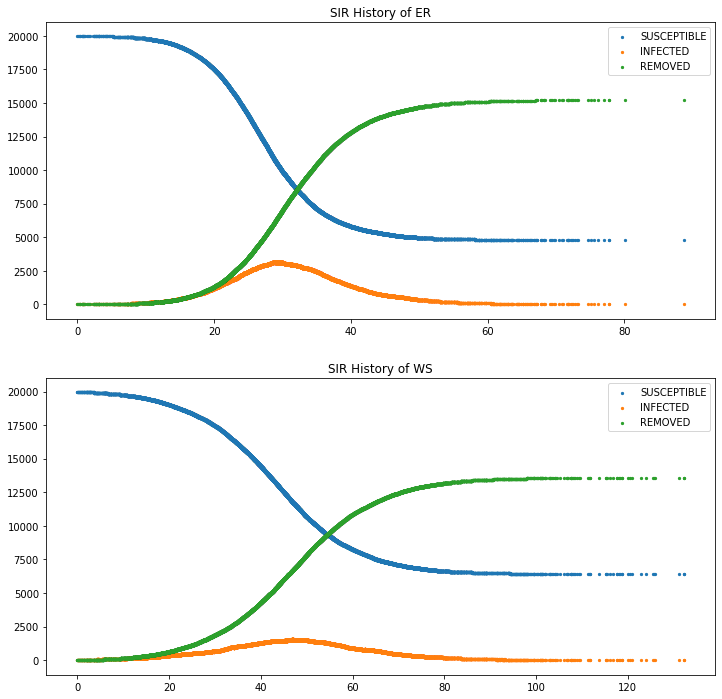
\includegraphics[scale=0.6]{images/ER_WS.png}
\end{center}
\newpage

\subsection{Scale Invariance (or the lack of it thereof)}
\subsubsection{Scale Invariance in ER Graph}
Infected proportion is plotted below for graph size 2k, 4k, 6k, 8k, 10k, 15k, 20k, 40k. They appear to be relatively close to each other in terms of the location and the magnitude of the peak, which is a sign of scale invariance.
\begin{center}
    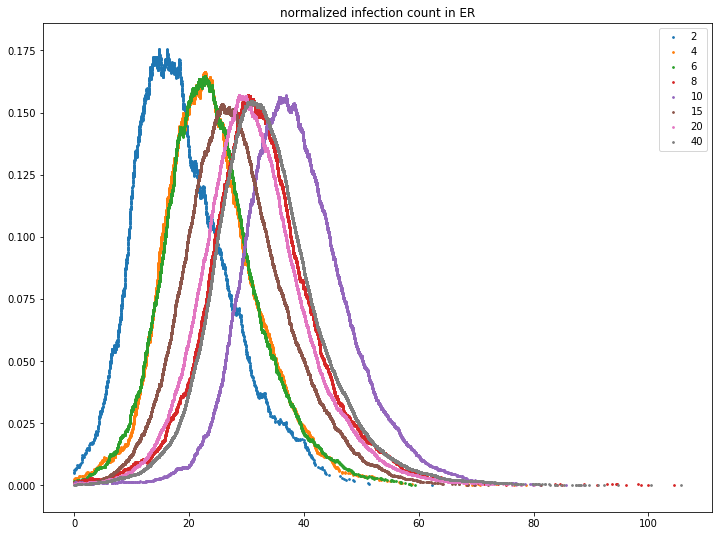
\includegraphics[scale=0.4]{images/ER_normalized.png}
\end{center}

\subsubsection{Lack of Scale Invariance in WS Graph}
Infected proportion is plotted below for graph size 1k, 2k, 5k, 10k, 20k. They vary greatly from each other in both the location and the magnitude of the peak. This justifies the need of realistic population count and is a property not exhibited by mean-field models. 
\begin{center}
    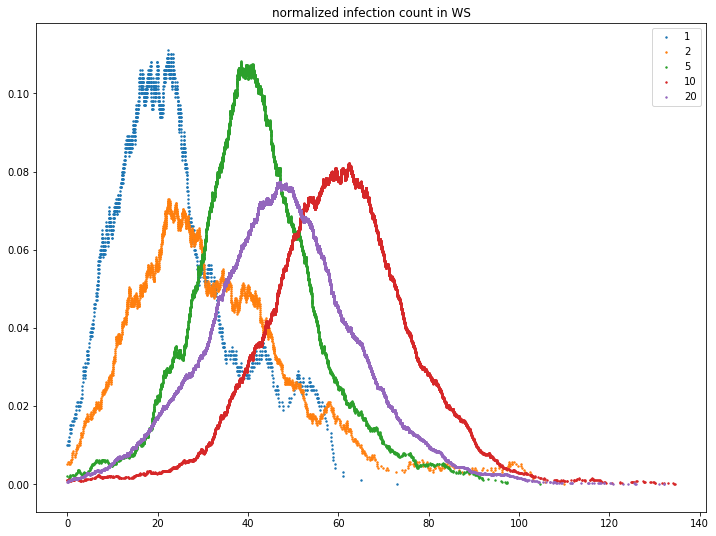
\includegraphics[scale=0.4]{images/WS_normalized.png}
\end{center}

\subsection{Impact of Different Rewiring Probability in WS Graph}
For a WS graph with 5000 nodes, the impact of different rewiring probability is examined. As rewiring probability $p$ goes up, the graph will be more like a random graph and less like a lattice.
\begin{center}
    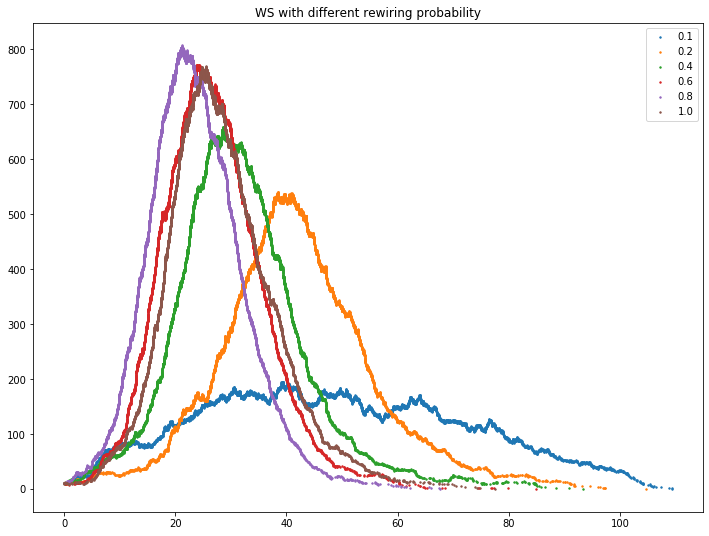
\includegraphics[scale=0.6]{images/rewiring.png}
\end{center}
Roughly speaking, increasing rewiring $p$ would result in an earlier and higher peak. This makes intuitive sense since as $p$ goes up, long-range travel would become more likely, speeding up infection. 

In a weird way, this looks awfully like the "FlattenTheCurve" figure. I guess the lesson here is that the society should really cut down on the disorder factor and be a good old lattice. 

\subsection{Comparison with the Mean-field SIR Model}
SIR Model without vital dynamics can be written as below
\begin{align*}
    \begin{cases}
        \dot{S} = -\beta SI\\
        \dot{I} = \beta SI - \gamma I\\
        \dot{R} = \gamma I\\
        S+I+R = 1
    \end{cases}
\end{align*}
We can find the peak of infection by setting 
\[\dot{I} = (\beta S - \gamma) I \triangleq 0\]
which implies that $S^* = \gamma / \beta$ at peak. In our settings, $S^* = \frac{1}{4.1 * 0.56} = 0.4355$

By visual inspection on the plot of 3.1, 
\begin{align*}
    S^*_{ER} \approx 10000/20000 = 0.5\\
    S^*_{WS} \approx 12500/20000 = 0.625
\end{align*}
Erdos-Renyi graph would then result in a better fit with mean-field SIR model. 

\bibliographystyle{plain}
\bibliography{report.bib}
\end{document}